\section{实验及分析}

本章节的实验环节使用与前一章节相同的有标记数据集。首先,本研究设置了一组对照实验,通过准确度和时间度量对比在不同数据集下不同图网络模型的结果值,用于探究模型在横向和纵向两个维度下对异常检测性能的提升效果;由于模型包含数个参数值,本章节还设置了多组步进参数的参数分析实验,以探究模型在参数选取上对异常检测结果的影响;最后,为了证实模型引入的几个关键方法的有效性,本文设置了一组消融实验,将其各部分与对应的基线函数进行了比较。

\subsection{数据集设置}

为了验证使用了基于路径的采样方法的具体表现,本章实验使用未经预处理的大型互联网路由数据集,具体地,本章实验使用 RIPE RIS 在 2017 和 2022 的两个路由异常事故中带有具体异常时间标记的真实路由数据集作为模型的输入,同时使用了 2022 年有异常标记的 DN42 路由数据集作为小批量数据的输入对照,一些基本参数已在先前的表 \ref{c3_data_input} 中列出。

\subsection{对比实验}

\subsubsection{实验设置}

作为对照,本章节将使用 GraphSAGE 模型和传统的 GCN 模型,在上述数据集中进行比较,将异常标记时间段1天前的数据作为参考输入进行模型的训练,然后将异常标记时间内的流式路由更新数据作为对照的异常检测的输入数据。此实验使用异常检测精确度和 F-1 作为模型评价指标,以异常分数 0.5 为异常阈值进行判断。除此之外,为了反映性能上的提升,还将统计实验完整运行(包括图网络构建/生成、图的嵌入、异常检测等步骤)的平均耗时作为运行效率提升的衡量指标。

在图的采样上,采用 $\theta_{sample} = \theta_{loss} = 1$ 的方式进行采样,即对图结构与路径两类因素赋予相同的权重,并设置采样规模 $N_{sample} = 6$。

\subsubsection{实验结果}
% 耗时

在完整运行上述模型后,将异常检测结果汇总统计,表格 \ref{c4_s3tab1} 展示了不同模型在x种数据集下的性能表现和对应的效率表现,由此可以得到以下发现:

\begin{enumerate}
    \item 本章模型在各数据集上的异常检测效果均优于原始模型,与 GCN 模型接近,对比常规 GraphSAGE 模型而言有接近 10\% 的提升,这说明了模型在引入路径特征之后具有更好的异常检测性能。
    \item 本章模型和常规 GraphSAGE 模型的运行效率相近,相比 GCN 模型而言,依然能够保证有较大的运行效率提升,证明了模型的采样方法是高效的。
    \item 模型在 DN42 分布式网络数据集中的表现不如在 RIPE RIS 互联网数据集,一种可能的解释是在分布式网络数据自身在不同节点上的属性相似度较高,因而路由路径数据对邻居相似度的影响相比更弱。
\end{enumerate}

\begin{table}
    \caption{对比实验结果}
    \begin{tabular}{lccccccccc}
        \toprule
                  & \multicolumn{3}{l}{RIPE.2017} & \multicolumn{3}{l}{RIPE.2022} & \multicolumn{3}{l}{DN42.2022}                                               \\ \cmidrule(lr){2-4} \cmidrule(lr){5-7} \cmidrule(lr){8-10}
        模型        & Acc.                          & F-1                           & 运行时间                          & Acc.  & F-1   & 运行时间 & Acc.  & F-1   & 运行时间 \\ \midrule
        GCN       & 0.821                         & 0.817                         & 732s                          & 0.832 & 0.829 & 769s & 0.791 & 0.780 & 25s  \\
        GraphSAGE & 0.779                         & 0.763                         & 112s                          & 0.785 & 0.771 & 114s & 0.742 & 0.725 & 12s  \\
        本章模型      & 0.846                         & 0.837                         & 162s                          & 0.836 & 0.820 & 165s & 0.803 & 0.794 & 19s  \\
        \bottomrule
    \end{tabular}
    \label{c4_s3tab1}
\end{table}

\subsection{参数分析}

模型在上述对比实验中设置了对应的采样规模 $N_{sample}$、采样参数 $\theta_{sample}$ 和损失计算参数 $\theta_{loss}$,为了研究不同参数对结果的影响,以及研究最佳的参数值的决定方式,本文还对该模型进行了参数分析实验。

\subsubsection{实验设置}

在本实验中,在模型的训练阶段,上述三个参数将被分别以一定的步进独立地进行调整,在调整具体某个参数时,其它参数将被固定在对比实验的默认值,训练好的模型将被输入已被标记为异常的时间段内的路由更新,以进行路由异常的检测。本次实验采用 RIPE RIS 在 2022 年带标记的路由异常事故中的数据集,模型同样采用异常发生1天前的数据作为正常训练样本。

\subsubsection{实验结果}

通过以上方式进行实验,将数据汇总至如图 \ref{c4_arg-result} 所示的折线图内,从图中能够针对模型的参数得出几个结论:

\begin{enumerate}
    \item 在一定范围内,提升采样规模 $N_{sample}$ 有助于提升模型性能,这实质上是通过增大采样子图的尺寸来实现的,在极端状况($N_{sample}$足够大)下的模型与一般消息传递的图神经网络无异,因而此参数的提升将增加图网络的计算量且存在饱和的可能。
    \item 在采样参数 $\theta_{sample}$ 和损失参数 $\theta_{loss}$ 上,可见存在与数据集对应的最优值,这是由于数据集自身在节点嵌入属性上具有的与路径和图网络的相关性决定的。
    \item $\theta$ 参数在一定范围内的增加均有助于提升模型的表现,这反映了本章模型引入数据集中基于路径特征的权重的必要性。
\end{enumerate}

\begin{figure}[h]
    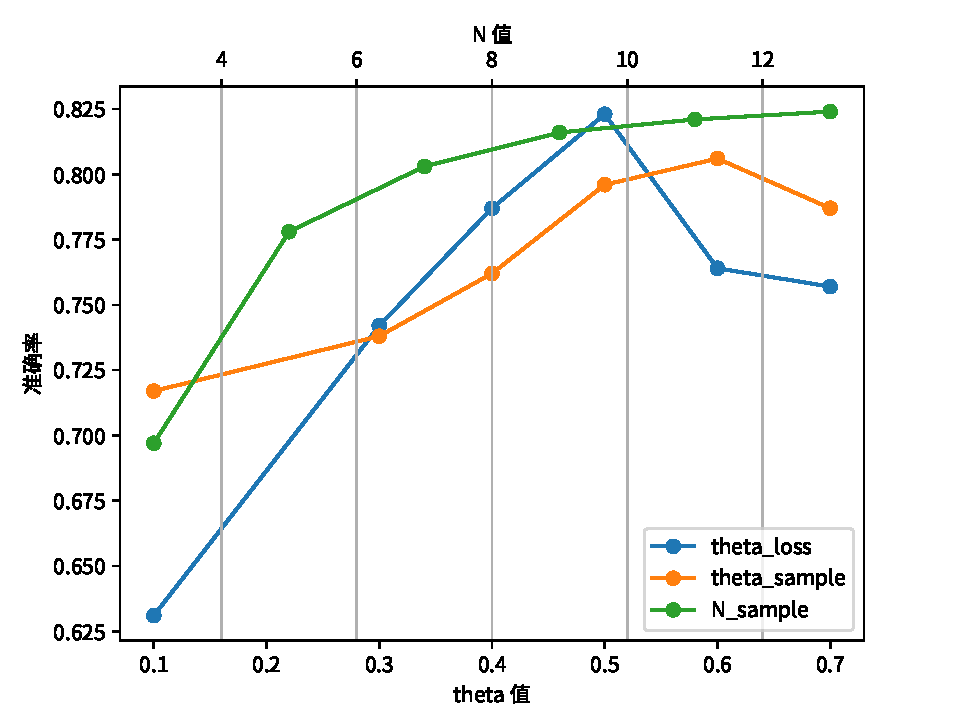
\includegraphics[width=0.9\linewidth]{chapter/c4_images/c4_arg-result.pdf}
    \caption{参数分析实验结果}
    \label{c4_arg-result}
\end{figure}

\subsection{消融实验}

本研究在 GraphSAGE 模型的基础上引入了独特的几种采样、聚合和计算损失的方式,为了验证其有效性,本研究为该模型设置了一组消融实验,该实验将展示这几类引入的算法在何种程度上提升了模型的最终效果。

\subsubsection{实验设置}

在消融实验中,作为对本章所述模型的消融对比,将在 GraphSAGE 模型的基础上替换采样函数、聚合函数和损失函数为各类基线函数,并采用与本章对比实验一致的参数设置,使用同样的数据集进行训练和测试。

实验一共针对模型中的三部分各自设置了三组对照:

\begin{enumerate}
    \item 对于邻居采样方法,设置了完全随机采样和以路径数量采样两种对照方法,对应研究在未引入路径因素和仅考虑路径因素的采样方法的条件下模型的性能变化。
    \item 针对聚合函数,设置了两组在 GraphSAGE 中常用的聚合方法\citing{hamilton2017inductive}作为对照,分别是均值聚合函数和归纳式均值聚合函数。
    \item 对于损失函数,消融实验设置了基于邻居嵌入最小化距离和路径嵌入最小化距离两种对照函数,分别对应于本模型中损失函数的两个极端情况。
\end{enumerate}

\subsubsection{实验结果}

消融实验的结果如表格 \ref{c4_s3tab2} 所示,它反映出了如下的一些特点:

\begin{enumerate}
    \item 本研究引入的基于路径的采样函数、聚合函数和损失函数均在提升异常检测性能上有一定贡献,总的来说,同时引入以上三种方式的模型的提升相比更大,这说明了本章在 GraphSAGE 三个方向提出的方法均在提升异常检测效果上具有作用。
    \item 在损失函数中引入基于路径的因素对模型的影响相比而言更大,一种可能的解释是,损失函数决定了训练参数的目标值,而采样和聚合方法自身在原理具有一定的随机性,从而在模型检测效果上的提升相对较少。
    \item 合理的设置参数 ($\theta$) 能够更好的提升模型异常检测的性能,这是由于在恰当的参数设置下,模型同时引入了路径和图的拓扑上的特征,过大或过小地设定参数将导致单一因素占据决定性比重,从而失去部分特征提取能力。
\end{enumerate}

\begin{table}
    \caption{消融实验结果}
    \begin{tabular}{lcccccc}
        \toprule
                        & \multicolumn{2}{l}{RIPE.2017} & \multicolumn{2}{l}{RIPE.2022} & \multicolumn{2}{l}{DN42.2022}                                                    \\ \cmidrule(lr){2-3} \cmidrule(lr){4-5} \cmidrule(lr){6-7}
        模型              & Acc.                          & F-1                           & Acc.                          & F-1            & Acc.           & F-1            \\ \midrule
        本章所述模型          & \textbf{0.846}                & \textbf{0.837}                & \textbf{0.836}                & \textbf{0.820} & \textbf{0.803} & \textbf{0.794} \\
        \midrule
        邻居采样                                                                                                                                                               \\
        \quad 完全随机采样    & 0.762                         & 0.759                         & 0.774                         & 0.771          & 0.750          & 0.752          \\
        \quad 以路径数量采样   & 0.795                         & 0.783                         & 0.799                         & 0.791          & 0.773          & 0.762          \\
        \midrule
        聚合函数                                                                                                                                                               \\
        \quad 均值聚合函数    & 0.749                         & 0.747                         & 0.752                         & 0.748          & 0.733          & 0.731          \\
        \quad 归纳式均值聚合函数 & 0.745                         & 0.743                         & 0.746                         & 0.744          & 0.730          & 0.735
        \\
        \midrule
        损失函数                                                                                                                                                               \\
        \quad 基于邻居嵌入最小化 & 0.721                         & 0.732                         & 0.725                         & 0.731          & 0.734          & 0.720          \\
        \quad 基于路径嵌入最小化 & 0.793                         & 0.790                         & 0.785                         & 0. 783         & 0.784          & 0.776
        \\
        \bottomrule
    \end{tabular}
    \label{c4_s3tab2}
\end{table}